% !TEX program = xelatex
%\documentclass[11pt,letterpaper]{article}
%\usepackage{beamerarticle}
\documentclass{beamer}

\usepackage{analchem}
\usepackage{lecture}
\usepackage{pdfpages}
\usepackage{ccicons}

\title{The Analytical Process}
\author{D.A.\ McCurry}
\institute[Bloomsburg University] % (optional)
{Department of Chemistry and Biochemistry\\
  Bloomsburg University}
\subtitle{Chapter 0}
\date{Fall 2020}

\begin{document}

\mode<presentation>{

\begin{frame}<handout:0>{Welcome to Analytical Chemistry I!}
%	\centering
%	\includegraphics[width=0.8\textwidth]{sewage.png}
%
%	\footnotetext{\tiny
%	\url{http://www.nydailynews.com/new-york/suburban-floaters-spoil-triathlon-article-1.1133003}}
%\end{frame}
	\centering

	\includegraphics[width=\linewidth]{lasvegas.png}
\end{frame}

\begin{frame}{Why is analytical chemistry important?}
	\begin{center}
		\includegraphics[width=0.9\linewidth]{Map_of_US_state_cannabis_laws.png}
	\end{center}
	\footnotetext{\ccbysa\ Lokal\_Profil}
\end{frame}

\begin{frame}{Some facts about THC}
	\begin{center}
		\includegraphics[scale=0.4]{THC.png}
	\end{center}

	\begin{itemize}
		\item Fat soluble -- it leaches out over time.
		\item Experienced users may not be affected as much as new or
			occasional users.
		\item THC can be detected long after impairment wears off.
	\end{itemize}

	\pause

	\begin{center}
		How can you \emph{objectively} detect driver impairment?
	\end{center}

	\footnotetext{https://cen.acs.org/articles/94/i13/Working-help-police-detect-drugged.html}
\end{frame}

\begin{frame}{A ``Breathalyzer-Type Instrument''}
	\centering

	\only<1>{\includegraphics[width=\linewidth]{THC-TOC.jpeg}}

	\pause
	
	\only<2->{\includegraphics[width=\linewidth]{THC-breathalyzer.jpeg}}

	\pause

	\bigskip

	What issues might this device have?

	\footnotetext{Hwang, S. I. et al. \textit{ACS Sens.} \textbf{2019}, 4
	(8), 2084–2093.}
\end{frame}

\begin{frame}
	\includegraphics[width=\linewidth]{shimadzu-cannabis.png}

	\footnotetext{https://www.ssi.shimadzu.com/industry/cannabis-testing-solutions.html
	(August 26, 2019)}
\end{frame}


}

\maketitle
\mode<article>{\thispagestyle{fancy}}

\begin{frame}
	\section{What is Analytical Chemistry?}
	\begin{learningobjectives}
		\item Understand the difference between qualitative and quantitative analysis.
		\item Know the steps for adequate chemical analysis.
	\end{learningobjectives}
\end{frame}

\begin{frame}{Chemical Analysis}
	Analytical chemistry deals with the
	identification and separation of materials \alert{and} the
	determination of its relative amount.

	\vspace{1em}

	\begin{figure}[h]
		\centering
		\sffamily
		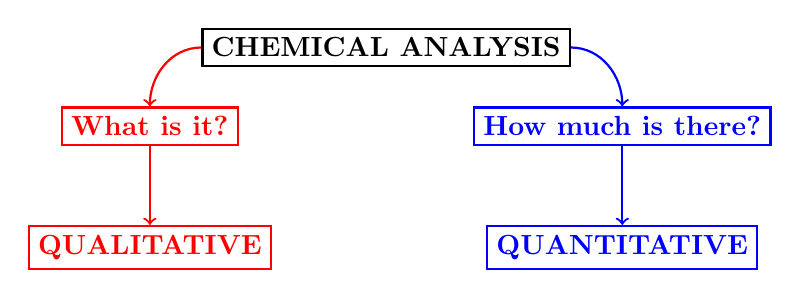
\begin{tikzpicture}
			\node[draw,thick](title) at (0,0) {\bfseries CHEMICAL
				ANALYSIS};
			\visible<2->{
				\node[draw,thick,red](qual) at (-3,-1)
				{\bfseries What is it?};
				\draw[->,thick,red] (title.west) to
				[in=90,out=180] (qual.north);
				\node[draw,thick,blue](quant) at (3,-1)
				{\bfseries How much is there?};
				\draw[->,thick,blue] (title.east) to
				[in=90,out=0] (quant.north);
				}
			\visible<3->{
				\draw[->,thick,red] (qual.south) to ++(0,-1)
				node[below,draw,thick,red]{\bfseries
				QUALITATIVE};
				\draw[->,thick,blue] (quant.south) to ++(0,-1)
				node[below,draw,thick,blue]{\bfseries
				QUANTITATIVE}; 
				}
		\end{tikzpicture}
	\end{figure}
\end{frame}

\begin{frame}{Steps in Chemical Analysis}
	\begin{overlayarea}{\linewidth}{0.85\textheight}
	\begin{enumerate}[<+->]
		\item \textbf{Formulate a Question}

			\only<1>{General questions into specific
			questions amenable to being answered through chemical
			measurements.
			
			\begin{itemize}
				\item<1> What amount of Pb is in our
					drinking water?
				\item<1> Will this plastic release harmful
					chemicals over time?
			\end{itemize}
			}
		
		\item \textbf{Select Analytical Procedure(s)}

			\only<2>{Search the chemical (scientific) literature to
			find appropriate procedures or, if necessary,
			\alert{develop original procedures} to make the required
			measurements.
			
			\begin{itemize}
				\item<2> What \alert{sensitivity} do we need?
				\item<2> How much \alert{analyte} will we have?
				\item<2> Will there be any \alert{interfering
					species}?
				\item<2> Which method is most
					\alert{cost-effective}?
			\end{itemize}
			}

		\item \textbf{Sampling}

			\only<3>{Obtain a representative bulk sample from the
			lot.
	
			\begin{itemize}
				\item<3> In most cases, it is \emph{impossible}
					to analyze \emph{every} sample.
			\end{itemize}
			}

		\item \textbf{Sample Preparation}

			\only<4>{Samples generally need to be purified, diluted,
			or even concentrated.
			
			\begin{itemize}
				\item<4> If we expect a \emph{really small}
					concentration, how do we detect it?
				\item<4> From the textbook, how do we analyze
					\emph{solid} chocolate bars via \alert{HPLC (High
					Performance \emph{Liquid}
					Chromatography)}
			\end{itemize}
			}

		\item \textbf{Analysis}

			\only<5>{Measure the concentration in \alert{several
			aliquots} of sample against a \alert{calibration} or
			\alert{standard curve}.

			\begin{itemize}
				\item<5> What happens if we make a mistake?
				\item<5> Can instruments make mistakes?
			\end{itemize}
			}

		\item \textbf{Reporting and Interpretation}

			\only<6>{Deliver a clearly written, complete report of
			your results \alert{highlighting any limitations that you
			attach to them}.
			
			\begin{itemize}
				\item<6> I'm grading your work.
				\item<6> More importantly, your post-graduation
					work will be read by others (bosses,
					legislators, \ldots)
			\end{itemize}

			\begin{alertblock}<6>{Note:}
			The report \alert{must} be appropriate for its
			intended audience.
			\end{alertblock}
			}

		\item \textbf{Drawing Conclusions}
			
			\only<7>{The more clearly a report is written, the
			less likely it is to be misinterpreted by those who use
			it.
			
			\begin{alertblock}<7>{Note:}
			Conclusions \alert{must} be consistent with the
			data.
			\end{alertblock}}
	\end{enumerate}
	\end{overlayarea}
\end{frame}

\begin{frame}{Constructing a Representative Sample}
	\begin{itemize}
		\item Chemical analysis is meaningless if we cannot demonstrate
			that the sample is \alert{representative} of the
			population.
		\item What factors influence the validity of the data?
	\end{itemize}

	\begin{center}
		\includegraphics[width=\linewidth]{box0-1.png}
	\end{center}
\end{frame}

\begin{frame}
	\begin{center}
		\includegraphics[width=0.8\linewidth]{RadNet-US.png}
	\end{center}
	\let\thefootnote\relax\footnotetext{\url{https://www.epa.gov/radnet/near-real-time-and-laboratory-data-state}}
\end{frame}

\begin{frame}
	\centering
	\includegraphics[width=0.95\linewidth,page=1]{CostNews2012Nov.pdf}
\end{frame}

%\mode<article>{\includepdf[pages=1]{CostNews2012Nov.pdf}}

\end{document}
